\documentclass[11pt,a4paper]{article}
\usepackage[margin=2.5cm]{geometry}
\usepackage{amsmath,amssymb,amsthm,mathtools}
\usepackage{booktabs,array,graphicx,xcolor}
\usepackage[colorlinks=true,linkcolor=blue!60!black,citecolor=green!40!black,urlcolor=blue!60!black]{hyperref}

\newcommand{\La}{\textsf{\textbf{(a)}}}
\newcommand{\Lb}{\textsf{\textbf{(b)}}}
\newcommand{\Lc}{\textsf{\textbf{(c)}}}
\newcommand{\Ld}{\textsf{\textbf{(d)}}}
\newcommand{\script}[1]{\texttt{scripts/#1}}
\newcommand{\Res}{\operatorname{Res}}
\newtheorem{proposition}{Proposition}[section]
\theoremstyle{remark}
\newtheorem{remark}[proposition]{Remark}

\title{Classical solitons of the Boussinesq equation:\\ a review with a view to quantisation}
\author{Project \emph{quantum\_boussinesq\_solitons}, Phase 1}
\date{3 November 2026}

\begin{document}
\maketitle

\begin{abstract}
We review the classical soliton theory of the Boussinesq equation in a single fixed convention. The emphasis is on the features that distinguish it from KdV-type and relativistic soliton theories, since these could obstruct or alter quantisation. We cover:
\begin{itemize}
\item the relations among the ``good'', ``bad'' and potential forms, the third-order Lax and $3\times3$ zero-curvature representations, the KP reduction, the $\mathfrak{sl}_3$ Gelfand--Dickey and classical $W_3$ structures, the Toda-lattice limit and the Hirota bilinear form;
\item one-soliton, $N$-soliton, breather, singular and resonant (merging) solutions;
\item a uniformising ``rapidity'' $\alpha$ with $k=\sin\alpha$, in which the two-soliton interaction constant is an explicit trigonometric function of $\alpha_1\pm\alpha_2$;
\item conserved charges on solitons, the soliton dispersion relation $E(P)$, and the structure of the soliton moduli space.
\end{itemize}
Every claim carries a status label: \La\ proved in the literature, \Lb\ conjectured or heuristic in the literature, \Lc\ derived in this project, \Ld\ a guess. All explicit formulas marked \Lc\ are verified by the scripts in \texttt{phase1/scripts}, listed in Appendix~\ref{app:checks}. Several results appear to be new or at least not stated in the literature we found; they are flagged as such. These are: the closed forms~\eqref{eq:Aov}--\eqref{eq:Aho}, the absence of regular breathers in the good equation, the bounded soliton momentum with a cusp at $k=\sqrt3/2$, and the degeneration of the induced symplectic form on the one-soliton manifold.
\end{abstract}

\tableofcontents

%======================================================================
\section{Conventions and summary}\label{sec:conv}

\paragraph{Fixed convention.} Throughout, ``Boussinesq'' means the \emph{good} equation
\begin{equation}\label{eq:good}
u_{tt}=u_{xx}-u_{xxxx}-3(u^2)_{xx},\qquad u=2(\log\tau)_{xx},\qquad (D_t^2-D_x^2+D_x^4)\,\tau\cdot\tau=0 ,
\end{equation}
and the \emph{bad} equation is
\begin{equation}\label{eq:bad}
v_{tt}=v_{xx}+v_{xxxx}+3(v^2)_{xx},\qquad v=2(\log\tau)_{xx},\qquad (D_t^2-D_x^2-D_x^4)\,\tau\cdot\tau=0 .
\end{equation}
The sign of the nonlinear term is conventional ($u\to-u$). Ours is fixed so that solitons are positive. This was checked in \script{../../phase0/checks/convention\_check.py} and \script{hirota\_solitons.py}. \Lc

\paragraph{Other papers' conventions.} The table records which equation each source uses and how it maps to ours. ``Good'' means $u_{tt}$ and $u_{xxxx}$ appear with opposite signs when both are written on the same side.

\begin{center}\small
\begin{tabular}{@{}p{4.6cm}p{6.4cm}p{3.6cm}@{}}
\toprule
Source & Equation as written & Type, map to ours\\\midrule
Bonnemain--Doyon \cite{BD} & $u_{tt}-u_{xx}=-\alpha[6(u^2)_{xx}+u_{xxxx}]$ & $\alpha=1$ good, $\alpha=-1$ bad; $u_{\rm BD}=u/2$\\
Corrigan--Zambon \cite{CZ} & $c^{-2}w_{tt}-w_{xx}-\lambda(w^2)_{xx}+\kappa^2w_{xxxx}=0$ & good\\
Rasin--Schiff \cite{RS}, Dimakis et al.\ \cite{DMHC} & $U_{tt}-4\beta U_{xx}+\tfrac13U_{xxxx}-2(U^2)_{xx}=0$ & good\\
Charlier--Lenells \cite{CL-GB} & $u_{tt}+\tfrac43(u^2)_{xx}+\tfrac13u_{xxxx}=0$ & good, zero background\\
Charlier--Lenells \cite{CL-WW,CL-SOL,CL-SR} & $u_{tt}=u_{xx}+(u^2)_{xx}+u_{xxxx}$ & \textbf{bad}\\
Bogdan--Charkina \cite{BC} & $w_{tt}-w_{xx}-w_{xxxx}+3(w^2)_{xx}=0$ & \textbf{bad}, $w=-v$\\
Clarkson--Dowie \cite{CD} & $u_{tt}+u_{xx}-(u^2)_{xx}-\tfrac13u_{xxxx}=0$ & bad on background $v_\infty=-\tfrac13$ (\S\ref{sec:rational})\\
Bazhanov--Hibberd--Khoroshkin \cite{BHK} & $L=\partial^3+u\partial+w$, chiral, periodic & $W_3$ form; no choice arises\\
\bottomrule
\end{tabular}
\end{center}

\paragraph{Summary of findings relevant to quantisation.}
\begin{enumerate}
\item \textbf{Good versus bad} is the choice of real or imaginary time in the second $\mathfrak{sl}_3$ Gelfand--Dickey flow (\S\ref{sec:lax}). \Lc\ The two equations have very different soliton content:
  \begin{itemize}
  \item good: subsonic solitons, a resonant and singular part of the two-soliton parameter space, and \emph{no regular breathers} (\S\ref{sec:breathers}); \Lc
  \item bad: supersonic solitons, regular interactions, and regular breathers. \La~\cite{CL-SOL,BC}
  \end{itemize}
\item Two-soliton phase shifts depend on \emph{both} $\alpha_1+\alpha_2$ and $\alpha_1-\alpha_2$~\eqref{eq:Aov}--\eqref{eq:Aho}. The equation has no boost symmetry, so a two-body S-matrix cannot be a function of a single rapidity difference. \Lc
\item ``Pure'' solitons do not exhaust the soliton content. There are resonant solutions in which two solitons merge into one (Y-junctions), and virtual solitons appear in head-on collisions. \La~\cite{HI,LMK,RS,DMHC} We identify the resonances as the zero and pole sets of~\eqref{eq:Aov}--\eqref{eq:Aho}. \Lc
\item Charges exist only at Gelfand--Dickey orders $n\not\equiv0\pmod 3$. \La\ On a soliton, every charge is a fixed linear combination of $\mu_1^m-\mu_2^m$, where $\mu_{1,2}$ are two roots of a cubic. \Lc
\item The one-soliton momentum of the good equation is bounded, $|P|\le\sqrt3/8$. $E(P)$ has two branches: a KdV-like light branch and a non-relativistic massive heavy branch. They meet at a cusp at $k=\sqrt3/2$, where the induced symplectic form on the one-soliton manifold degenerates. \Lc
\item In both forms the Hamiltonian is unbounded below. The bad equation is ill-posed, yet it is the form that arises as the continuum limit of the (quantisable) Toda lattice, and the only one for which a rigorous inverse scattering transform with solitons exists. \La/\Lc
\end{enumerate}

%======================================================================
\section{The equations and their relations}\label{sec:equations}

\subsection{Good, bad and potential forms}\label{sec:goodbad}

Plane waves $e^{i(kx-\omega t)}$ of the linearisations obey
\[
\omega^2=k^2+k^4 \ \text{(good)},\qquad \omega^2=k^2-k^4\ \text{(bad)} .
\]
The bad linearisation has modes with $|k|>1$ growing at rate $|k|\sqrt{k^2-1}$, which is unbounded. The Cauchy problem is therefore Hadamard ill-posed in Sobolev spaces. \La~\cite{BD,CL-WW}

Even so, Charlier and Lenells prove that the bad equation has a unique global Schwartz solution whenever the reflection coefficient $r_1$ vanishes on $[0,i]$ (``no unstable high-frequency modes''). They also construct solutions that blow up at any prescribed time $T$. \La~\cite[Thms 2.8--2.12]{CL-WW}, extended to solitons in \cite[Thms 2.6--2.11]{CL-SOL}.

For the good equation, local well-posedness and global existence for small data are classical. \La~\cite{BonaSachs} (abstract only seen.)

\paragraph{Formal map between the forms.} The substitution $x\to ix$, $t\to it$, $u\to-u$ maps~\eqref{eq:good} to~\eqref{eq:bad}. It does not preserve real solutions. On Hirota data it acts as $k\to ik$, $\omega\to i\omega$, which maps the soliton dispersion $\omega^2=k^2-k^4$ to $\omega^2=k^2+k^4$. \Lc

\paragraph{Potential and Lagrangian form.} With $u=\phi_x$, equation~\eqref{eq:good} is the Euler--Lagrange equation of
\begin{equation}\label{eq:Lag}
\mathcal L=\tfrac12\phi_t^2-\tfrac12\phi_x^2-\tfrac12\phi_{xx}^2+\phi_x^3 ,
\end{equation}
verified in \script{charges.py}. \Lc\ Equivalently, in first-order form, $u_t=w_x$, $w_t=(u-u_{xx}-3u^2)_x$.

The canonical momentum is $\pi=\phi_t$ with bracket $\{\phi(x),\pi(y)\}=\delta(x-y)$. The conserved mass, momentum and energy are
\begin{equation}\label{eq:EPM}
M=\int u\,dx,\qquad P=-\int \phi_t\,\phi_x\,dx,\qquad H=E=\int\Big(\tfrac12\pi^2+\tfrac12u^2+\tfrac12u_x^2-u^3\Big)dx .
\end{equation}
$P$ generates spatial translations, $\{\phi,P\}=-\phi_x$.

\paragraph{Unbounded energy.} Because of the cubic term, $H$ is unbounded below: take $u=\lambda f$ with $f\ge0$ fixed and $\lambda\to\infty$. \Lc\ (elementary) The bad Lagrangian has $+\tfrac12\phi_{xx}^2$, so its $H$ is unbounded below already at quadratic order. The same holds for Bogdan--Charkina's energy \cite[eq.\,(10)]{BC}. Both facts matter for quantisation (\S\ref{sec:wellposed}).

\subsection{Lax pair, real versus imaginary time, and the $3\times3$ zero-curvature form}\label{sec:lax}

Let
\[
L=\partial_x^3+q\,\partial_x+r,\qquad M=(L^{2/3})_+=\partial_x^2+\tfrac23 q .
\]
The Lax equation $L_\tau=[M,L]$ is equivalent to
\begin{equation}\label{eq:laxflow}
q_\tau=2r_x-q_{xx},\qquad r_\tau=r_{xx}-\tfrac23q_{xxx}-\tfrac23qq_x,
\qquad\Longrightarrow\qquad q_{\tau\tau}=-\tfrac13 q_{xxxx}-\tfrac23(q^2)_{xx}.
\end{equation}
This is the Lax pair of Zakharov \cite{Zak}; see also \cite[eqs.\,(1.7)--(1.8)]{CL-GB} for an equivalent form. The rewriting~\eqref{eq:laxflow} is verified in \script{lax\_zero\_curvature.py}. \La/\Lc

\begin{proposition}[\Lc, \script{lax\_zero\_curvature.py}]\label{prop:goodbad}
Set $q=\tfrac32u-\tfrac14$ and $\tau=\sqrt3\,t$ (real Lax time). Then~\eqref{eq:laxflow} is exactly the good equation~\eqref{eq:good}.

Set instead $q=\tfrac32v+\tfrac14$ and $\tau=i\sqrt3\,t$. Then it is the bad equation~\eqref{eq:bad}.

In both cases the $u_{xx}$ (sound) term comes entirely from the constant background $q_\infty=\mp\frac14$.
\end{proposition}

So both equations are the same complexified flow on the same phase space of third-order operators. They differ in the real form chosen for time and in the background. This is why the chiral $W_3$ conformal field theory literature never has to choose (\S\ref{sec:w3}).

\paragraph{Zero-curvature form.} Writing $L\psi=\lambda\psi$ as a first-order system for $\Psi=(\psi,\psi_x,\psi_{xx})^T$ gives
\[
\Psi_x=U\Psi,\qquad U=\begin{pmatrix}0&1&0\\0&0&1\\\lambda-r&-q&0\end{pmatrix},\qquad \Psi_\tau=V\Psi .
\]
The rows of $V$ are generated from $\psi_\tau=M\psi$. Then $U_\tau-V_x+[U,V]=0$ holds identically on solutions of~\eqref{eq:laxflow}. \Lc\ (verified)

$U$ is of Drinfeld--Sokolov type: a principal nilpotent element plus $\lambda$ times the lowest root vector of $\mathfrak{sl}_3$, plus a lower-triangular potential. \La~\cite{DS}

The rigorous inverse scattering transforms \cite{CL-GB,CL-WW,CL-SOL} work with gauge-equivalent $3\times3$ systems. Their spectral variable is uniformised by $k$ with $\lambda\propto k^3$ (good, \cite[(3.1)]{CL-GB}) or $\lambda=(k^3+k^{-3})/2$ (bad, \cite[(3.2)]{CL-WW}). Their jump contours carry the $\mathbb Z_3$ symmetry $k\mapsto\omega k$, $\omega=e^{2\pi i/3}$. \La

\paragraph{The spectral picture of a soliton.} This is the key structure used below.
\begin{itemize}
\item On the background $q=-\frac14$, $r=0$, the function $e^{\mu x}$ is an eigenfunction of $L$ with eigenvalue $\lambda=\mu^3-\mu/4$.
\item A soliton of wavenumber $k$ and velocity $v$ corresponds to two roots $\mu_1,\mu_2$ of $\mu^3-\mu/4=\lambda$ with
\begin{equation}\label{eq:mu}
\mu_1-\mu_2=k,\qquad \mu_1+\mu_2=-v/\sqrt3 .
\end{equation}
\item The condition that both are roots of the same cubic, $\mu_1^2+\mu_1\mu_2+\mu_2^2=\frac14$, is exactly $v^2=1-k^2$. \Lc\ (\script{charges.py})
\item The three roots are $\mu_j=\frac1{\sqrt3}\sin(\varphi+2\pi j/3)$, $j=0,1,2$, for $\lambda=-\sin(3\varphi)/(12\sqrt3)$.
\end{itemize}
A soliton is therefore an \emph{ordered pair of sheets} of a three-sheeted spectral curve. Left- and right-movers are different pairs. This is the classical counterpart of the $\mathfrak{sl}_3$ weight labelling of affine Toda solitons \cite{Hol92}. \Lc\ (structure), \Ld\ (significance)

The same structure appears as $P^3=3\beta P+C$ in \cite[(2.8)]{DMHC} and as $\lambda^3=3\beta\lambda+\theta$ in \cite[§3]{RS}. \La

\subsection{KP and Gelfand--Dickey reduction; bi-Hamiltonian structure and classical $W_3$}\label{sec:w3}

\paragraph{KP reduction.} With $q=\tfrac32w$, the static ($T$-independent) KP-II equation
\[
(4w_T-6ww_x-w_{xxx})_x=3w_{yy}
\]
reduces to~\eqref{eq:laxflow} with $\tau=y$. \Lc\ (verified)

In hierarchy language, the Boussinesq hierarchy is the 3-reduction of the KP hierarchy: $\mathcal L^3=L$ is a differential operator. The flows are $\partial_{t_n}L=[(L^{n/3})_+,L]$. The $t_{3m}$ flows are trivial, and the Boussinesq equation is the $t_2$ flow. \La~\cite{Dickey}

In the KP picture the solitons are line solitons $e^{(p-q)x+(p^2-q^2)y}$. The reduction pairs the roots $p,q$ as in~\eqref{eq:mu}. \La~\cite{DMHC}

\paragraph{Charges and the missing spins.} The conserved charges are $H_n=\int\Res L^{n/3}\,dx$. They vanish identically for $n\equiv0\pmod3$, because $L^{m}$ is a differential operator. \La~\cite{Dickey} We verified directly that $\Res L^{3/3}=\Res L^{6/3}=0$ and that $\Res L^{n/3}\neq0$ for $n=1,2,4,5$. \Lc\ (\script{charges.py})

In $W_3$ language the charge $H_n$ has spin $n$, and its density has spin $n+1$. Hence there are charges of spins $1,2,4,5,7,8,\dots$ but none of spins divisible by 3. \La

This classical gap is reproduced at generic central charge in the quantum theory for the lowest spins \cite{KM}. At $c=-2$ there are quantum charges at \emph{all} spins $s\ge2$ \cite{Bordner}. \La

The same trichotomy appears in the Bäcklund-transformation conservation laws: those with index divisible by 3 are trivial \cite[eqs.\,(29)--(30)]{RS}. \La

\paragraph{Bi-Hamiltonian structure and $W_3$.} The Adler--Gelfand--Dickey construction gives two compatible Poisson brackets on $\{q,r\}$ \cite{Adler,Dickey}. The second bracket is the classical $W_3$ algebra:
\begin{itemize}
\item a Virasoro density $T\propto q$ (with a central term);
\item a spin-3 primary $W\propto r-\tfrac12q_x$.
\end{itemize}
\La~\cite{Mathieu88,MathieuOevel,BS}

The Boussinesq flow is Hamiltonian for both brackets: it is generated by $H_2$ for the second bracket and by $H_5$ for the first. \La~\cite{Dickey,MathieuOevel} We have not re-derived the bracket normalisations. Consistently with this, the physical energy~\eqref{eq:EPM} lies in the span of $H_5$ and $H_1$ on solitons (Prop.~\ref{prop:charges}). \Lc

The quantisation of the second bracket is the $W_3$ algebra. Its commuting charges are the quantum Boussinesq charges \cite{KM,Bordner,BHK,MR,Ashok1,Ashok2}. These all live in highest-weight modules on a circle (chiral conformal field theory), not on the line with asymptotic states. \La

\subsection{Toda lattice limit}\label{sec:toda}

Write the Toda lattice in strain variables $r_n=x_{n+1}-x_n$:
\[
\ddot r_n=2e^{-r_n}-e^{-r_{n+1}}-e^{-r_{n-1}} .
\]
\begin{proposition}[\Lc, \script{toda\_limit.py}]
To the Boussinesq order the continuum expansion is
\[
r_{tt}=r_{XX}+\tfrac1{12}r_{XXXX}-\tfrac12(r^2)_{XX}+\dots
\]
After $X=\xi/\sqrt{12}$, $t=s/\sqrt{12}$ and $r=-6v$ this is exactly the \emph{bad} equation~\eqref{eq:bad}.

The Toda two-soliton interaction constant is $A^{\rm T}=-P_{\rm T}(\kappa_1-\kappa_2,\omega_1-\omega_2)/P_{\rm T}(\kappa_1+\kappa_2,\omega_1+\omega_2)$, with $P_{\rm T}(\kappa,\omega)=\omega^2-4\sinh^2(\kappa/2)$. The exact Toda two-soliton solution was checked in the lattice equation to $10^{-17}$. As the amplitudes go to zero with $\kappa=\sqrt{12}k$, $\log A^{\rm T}/\log A^{\rm bad}\to1$ for both overtaking and head-on collisions; the ratio is $1+O(10^{-4})$ at $k\sim10^{-2}$.
\end{proposition}

That the Toda/FPU long-wave limit has the ill-posed sign is classical. \La~\cite{Zak,BC} The lattice cures the ill-posedness: the full Toda dispersion $\omega=2\sin(k/2)$ is bounded.

\emph{Implication.} The exactly solvable quantum Toda chain \cite{Sutherland,Gutzwiller,Sklyanin,Mertens,SiddharthanShastry,PustilnikMatveev} provides a well-defined quantum regularisation of the \emph{bad} Boussinesq soliton sector. \Ld, to be pursued in Phase~2, Route~D.

\subsection{Hirota bilinear form}

With $u=2(\log\tau)_{xx}$, equation~\eqref{eq:good} follows from $(D_t^2-D_x^2+D_x^4)\tau\cdot\tau=0$. \La~\cite{Hirota73} We verify this for every explicit solution below.

%======================================================================
\section{Soliton solutions}\label{sec:solitons}

\subsection{One-soliton}

The one-soliton solution of~\eqref{eq:good} is
\begin{equation}\label{eq:1sol}
\tau=1+e^{\theta},\quad \theta=kx-\omega t+x_0,\quad \omega=\epsilon k\sqrt{1-k^2},\qquad u=\frac{k^2}{2}\operatorname{sech}^2\frac{\theta}{2} .
\end{equation}
\begin{itemize}
\item Here $0<k<1$ and $\epsilon=\pm1$ (right- or left-moving).
\item The speed is $v=\sqrt{1-k^2}<1$: solitons are subsonic, and the \emph{larger ones are slower}.
\item The amplitude is at most $\frac12$, reached by the static soliton at $k\to1$.
\end{itemize}
\Lc\ (\script{hirota\_solitons.py}); cf.\ \cite[(18)]{BD} and \cite[(2.8)]{CZ}.

It is convenient to uniformise:
\begin{equation}\label{eq:alpha}
k=\sin\alpha,\qquad v=\cos\alpha,\qquad \omega=\tfrac{\epsilon}{2}\sin2\alpha,\qquad \alpha\in(0,\tfrac\pi2).
\end{equation}
Corrigan--Zambon use $\nu=\tanh\theta$, so $k=\operatorname{sech}\theta$ and $\alpha=\tfrac\pi2-\operatorname{gd}\theta$ \cite[(5.6)--(5.8)]{CZ}.

For the bad equation, $k=\sinh\beta$ and $v=\cosh\beta>1$: solitons are supersonic, with all amplitudes and speeds allowed. \La~\cite[(A.8)]{CL-SOL}, \cite[(11)]{BC}

Singular one-solitons, $\tau=1-e^\theta$ with $u=-\frac{k^2}2\operatorname{csch}^2\frac\theta2$, also solve~\eqref{eq:good}. \La~\cite{RS} In the inverse scattering transform for the bad equation, real zeros of $s_{11}$ give regular or singular solitons according to the sign of the residue constant. \La~\cite[Lemma A.3]{CL-SOL}

\subsection{\texorpdfstring{$N$}{N}-soliton solutions and the interaction constant}

\begin{equation}\label{eq:Nsol}
\tau=\sum_{\mu\in\{0,1\}^N}\exp\Big(\sum_i\mu_i\theta_i+\sum_{i<j}\mu_i\mu_j\log A_{ij}\Big),\qquad
A_{ij}=-\frac{\mathcal P(k_i-k_j,\omega_i-\omega_j)}{\mathcal P(k_i+k_j,\omega_i+\omega_j)} ,
\end{equation}
where $\mathcal P(K,W)=W^2-K^2+K^4$. Here $\theta_i=k_ix-\omega_it+x_i$ and $\omega_i=\epsilon_ik_i\sqrt{1-k_i^2}$. This is Hirota's construction \La~\cite{Hirota73}.

\emph{Checks.} \Lc
\begin{itemize}
\item The two-soliton was substituted directly into~\eqref{eq:good}: residual $<10^{-38}$ at 40-digit precision, for both overtaking and head-on configurations.
\item The bilinear Hirota condition holds \emph{exactly} for $N=2,3,4$ in all $2^N$ direction patterns, in rational arithmetic with Pythagorean $k$'s.
\item It holds to machine precision for complex (breather-type) parameters.
\item $A_{12}$ agrees with Bonnemain--Doyon's eq.\,(16) \cite{BD}, with their $\eta=k$.
\end{itemize}

\begin{proposition}[\Lc, \script{interaction\_regimes.py}]\label{prop:A}
Let $S=\alpha_1+\alpha_2$ and $D=\alpha_1-\alpha_2$. For the good equation,
\begin{align}
\text{overtaking } (\epsilon_1=\epsilon_2):&\quad A_{12}=\frac{1-3\cot^2(S/2)}{1-3\cot^2(D/2)}
=\frac{\sin(\frac S2+\frac\pi3)\sin(\frac S2-\frac\pi3)\,\sin^2\frac D2}{\sin(\frac D2+\frac\pi3)\sin(\frac D2-\frac\pi3)\,\sin^2\frac S2},\label{eq:Aov}\\
\text{head-on } (\epsilon_1=-\epsilon_2):&\quad A_{12}=\frac{1-3\tan^2(D/2)}{1-3\tan^2(S/2)} .\label{eq:Aho}
\end{align}
For the bad equation, with $\alpha\to i\beta$,
\begin{equation}
A^{\rm bad}_{\rm ov}=\frac{1+3\coth^2(S/2)}{1+3\coth^2(D/2)},\qquad A^{\rm bad}_{\rm ho}=\frac{1+3\tanh^2(D/2)}{1+3\tanh^2(S/2)} ,
\end{equation}
now with $S=\beta_1+\beta_2$ and $D=\beta_1-\beta_2$. Both bad constants lie in $(0,1)$.
\end{proposition}

Formula~\eqref{eq:Aov} has the same $\pm\pi/3$ shift structure as the $\mathfrak{sl}_3$ affine Toda interaction factors \cite{Hol92}. The difference is the simultaneous dependence on $S$ and $D$. The first factorised form is close to \cite[(5.8)--(5.9)]{CZ}. We have not found~\eqref{eq:Aov}--\eqref{eq:Aho} stated in this form elsewhere.

\begin{figure}[t]\centering
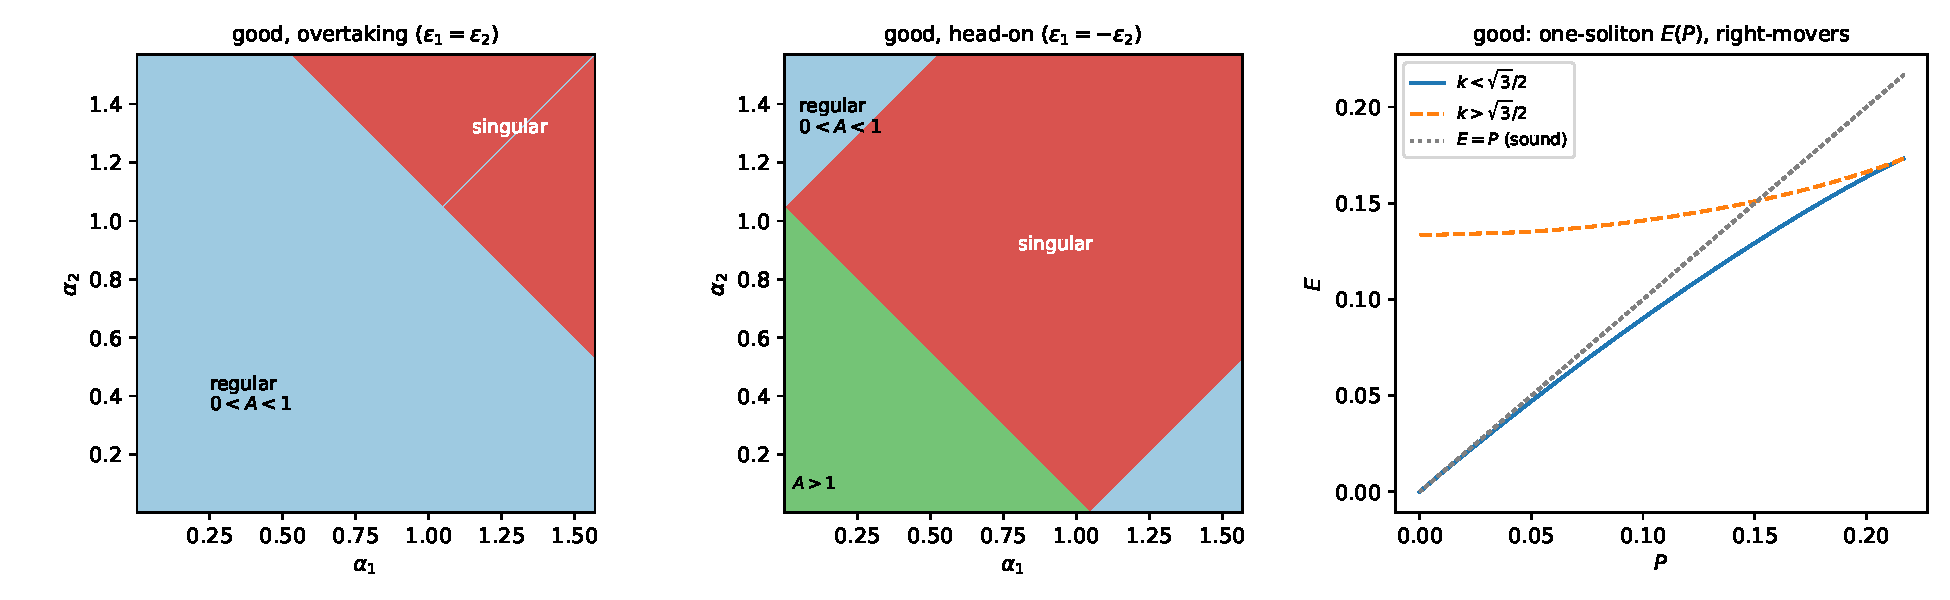
\includegraphics[width=\textwidth]{figures/regimes_and_dispersion.pdf}
\caption{\emph{Left and centre:} regularity of the good two-soliton solution in the $(\alpha_1,\alpha_2)$ plane (Prop.~\ref{prop:regimes}). Red: singular ($A<0$). Blue: regular and repulsive ($0<A<1$). Green: regular and attractive ($A>1$). The boundaries are resonance lines. \emph{Right:} the good one-soliton dispersion relation $E(P)$, with a light branch (solid) and a heavy branch (dashed) meeting at the cusp $k=\sqrt3/2$ (Prop.~\ref{prop:EP}).}\label{fig:regimes}
\end{figure}

\subsection{Regularity, resonances and merging solitons}\label{sec:resonance}

For real $\theta_i$, a two-soliton $\tau=1+e^{\theta_1}+e^{\theta_2}+A_{12}e^{\theta_1+\theta_2}$ is positive for all $(x,t)$ if and only if $A_{12}>0$. If $A_{12}<0$, $\tau$ vanishes along curves and $u$ is singular there.

\begin{proposition}[\Lc]\label{prop:regimes}
For the good equation the following hold; see Fig.~\ref{fig:regimes}.
\begin{enumerate}
\item \emph{Overtaking.} The solution is regular if and only if $\alpha_1+\alpha_2<\frac{2\pi}3$. Then $0<A<1$, so the interaction is repulsive. It is singular for $\alpha_1+\alpha_2>\frac{2\pi}3$. On the line $\alpha_1+\alpha_2=\frac{2\pi}3$ we have $A=0$.
\item \emph{Head-on.} There are three regions:
  \begin{itemize}
  \item regular and attractive ($A>1$) for $\alpha_1+\alpha_2<\frac\pi3$;
  \item regular and repulsive ($0<A<1$) for $|\alpha_1-\alpha_2|>\frac\pi3$;
  \item singular otherwise.
  \end{itemize}
  $A=\infty$ on $\alpha_1+\alpha_2=\frac\pi3$, and $A=0$ on $|\alpha_1-\alpha_2|=\frac\pi3$.
\item \emph{Resonance.} On every resonance line, the difference or sum $(k_1\mp k_2,\omega_1\mp\omega_2)$ satisfies the soliton dispersion relation $\mathcal P=0$. The degenerate $\tau$ (three exponentials) then describes a Y-junction in which two solitons merge into one, or one splits into two. The merging conserves $k$ and $\omega$.
\end{enumerate}
\end{proposition}

These regions agree with the conditions of Lambert, Musette and Kesteloot quoted in \cite[(29)--(33)]{BD}: with $\eta=\sin\alpha$, their bounds $\tfrac12|\eta\mp\sqrt{3(1-\eta^2)}|$ equal $\sin|\alpha\mp\pi/3|$. \Lc

Merging solitons were found by Hirota and Ito \cite{HI} and Lambert et al.\ \cite{LMK}, and rederived via Bäcklund transformations by Rasin and Schiff \cite{RS}. Rasin--Schiff's ``law of conservation of speed'' is $\lambda_1+\lambda_2+\lambda_3=0$ \cite[§3]{RS}. In~\eqref{eq:mu} this is the statement that the three solitons $(\mu_1\mu_2)$, $(\mu_2\mu_3)$, $(\mu_1\mu_3)$ of a Y-junction use the three roots of one cubic. \La\ for the solutions, \Lc\ for the identification.

The resonant interaction persists in the matrix case as an elementary rooted binary tree in the tropical limit \cite[Remark 3.4]{DMHC}. \La

\paragraph{Bonnemain--Doyon's sign conventions.} We find the position-shift sign conventions of \cite[(22) vs (24)]{BD} inconsistent, and their printed bilinear form \cite[(12)]{BD} carries the bad sign; both look like typos. Their eq.\,(16) itself is correct, as checked above. \Lc

\subsection{Breathers: none regular in the good equation}\label{sec:breathers}

A breather is the real reduction $k_2=\bar k_1$, $\omega_2=\bar\omega_1$ of the two-soliton. Write $\theta=R+iI$. Then
\[
\tau=1+2e^{R}\cos I+A(k,\bar k)\,e^{2R}.
\]
Since $I$ varies through all values, $\tau>0$ everywhere if and only if $A(k,\bar k)>1$.

\begin{proposition}[\Lc, \script{interaction\_regimes.py}]\label{prop:nobreather}
For the good equation~\eqref{eq:good} with $\alpha=a+ib$,
\[
A(k,\bar k)=\frac{1-3\cot^2a}{1+3\coth^2b}<\frac14 .
\]
Hence \emph{every Hirota breather of the good Boussinesq equation on the zero background is singular}. This is confirmed numerically on a grid in $\alpha$ (largest value $A=0.2365$) and by a scan of the complex $k$-plane.

For the bad equation, about $18\%$ of the scanned region $0<\operatorname{Re}k,\operatorname{Im}k<2$ gives $A>1$, i.e.\ regular breathers.
\end{proposition}

This is consistent with the following rigorous and literature results:
\begin{itemize}
\item For the bad equation, breathers from non-real zeros of $s_{11}$ in a region $D_{\rm reg}$ are smooth for all $t$. Those from $D_{\rm sing}$ have a singularity at \emph{every} time $t$. \La~\cite[Lemma A.4]{CL-SOL} The key quantity there is $\det(I-A)=1-2\operatorname{Re}A_{11}+h|A_{11}|^2$ with $h>4$ on $D_{\rm reg}$, which is the same structure as our $1-2X\cos I+AX^2$.
\item The Tajiri--Murakami breather of the bad equation exists exactly for $\pi/3<\beta\le\pi/2$ in Bogdan--Charkina's parametrisation $\kappa\pm ik=\sinh(\alpha\pm i\beta)$. At $\beta=\pi/3$ it degenerates into the linear localised mode of the kink. \La~\cite[(29)--(41)]{BC}
\end{itemize}

We did not find the statement that the good equation has no regular breathers in the literature. It concerns the two-phase Hirota class on zero background only. Breather-like structures on non-zero backgrounds \cite{BD} are not excluded.

\subsection{Rational solutions}\label{sec:rational}

Clarkson and Dowie construct algebraically decaying rational solutions $u=2(\log F)_{xx}$, with $F$ a special polynomial, of $u_{tt}+u_{xx}-(u^2)_{xx}-\tfrac13u_{xxxx}=0$. \La~\cite{CD} Their integral relations are studied in \cite{ABCD}.

By $u=3(v+\tfrac13)$ and $x=X/\sqrt3$, $t=T/\sqrt3$, this equation becomes the bad equation~\eqref{eq:bad} for $v$ on the background $v_\infty=-\tfrac13$. \Lc\ (\script{clarkson\_dowie\_map.py}) On that background the linearisation is $\omega^2=-k^2-k^4$, which is unstable for every $k$.

Rational solutions therefore do not live in the vacuum sector of either the good or the bad equation in real variables. They are irrelevant to scattering around the vacuum. \Lc

%======================================================================
\section{Features that distinguish Boussinesq solitons}\label{sec:features}

We assess each of the hints in the project brief, and add a few more.

\subsection{Singular versus nonsingular solutions}

\textbf{Verdict: true.} Regularity depends on spectral data in several independent ways:
\begin{itemize}
\item the sign of the residue constant, for one-solitons \cite[Lemma A.3]{CL-SOL} \La;
\item the location of the spectral parameters in the two-soliton problem (Prop.~\ref{prop:regimes}) \Lc;
\item breathers: singular for \emph{every} $t$ in $D_{\rm sing}$ for the bad equation \La~\cite{CL-SOL}, and \emph{always} singular for the good equation (Prop.~\ref{prop:nobreather}) \Lc.
\end{itemize}

In addition, Rasin--Schiff find superpositions of merging solitons that develop a singularity at a finite time and lose it later. This is numerical evidence, without classification. \Lb~\cite[Fig.\,8]{RS}

For the vector equation, every regular $N=2$ three-root solution has singular ones arbitrarily close to it. \La~\cite[Prop.\,3.7]{DMHC}

\subsection{Pure solitons do not exhaust the soliton content; virtual solitons}

\textbf{Verdict: true.} In the classification of \cite{DMHC}, ``pure solitons'' use one pair of roots per soliton. Unlike in the KdV case, they do not exhaust the solitons of the Boussinesq reduction \La~\cite[Intro, §3.3]{DMHC}. The others are the merging and splitting (Y-junction) solutions of \S\ref{sec:resonance}.

\emph{Virtual solitons.} In head-on collisions near resonance, an intermediate ``virtual'' soliton forms in the interaction region and then splits; this has no KdV counterpart \La~\cite[Fig.\,2]{DMHC}, \cite{HI}. Our reading agent checked that the parameters in that figure make $\tau$ a scalar Boussinesq $\tau$-function, so this is a scalar phenomenon. \Lc

In~\eqref{eq:Aho}, $\log A$ diverges at the resonances. For instance, as $|\alpha_1-\alpha_2|\to\frac\pi3$ we have $A\to0$, and the time spent in the virtual state grows logarithmically. \Lc

\subsection{Two-soliton scattering}

\begin{itemize}
\item \emph{Pairwise additivity.} By~\eqref{eq:Nsol}, asymptotic phase shifts in $N$-soliton solutions are sums of pairwise $\log A_{ij}$. Classical scattering of pure solitons is therefore factorised. \La/\Lc\ (Hirota condition verified for $N\le4$.)
\item \emph{Position shifts.} The position shift of soliton $i$ is $\pm k_i^{-1}\log A_{12}$. The sign is $+$ if soliton $i$ ends up on the side where the other soliton's phase is $+\infty$. This was checked against peak-tracking of the exact solution for overtaking, attractive head-on and repulsive head-on cases, to $\lesssim3\times10^{-3}$. \Lc
\item \emph{Dependence on orientation.} Overtaking collisions are always repulsive. Head-on collisions are attractive for small solitons ($\alpha_1+\alpha_2<\pi/3$) and repulsive for very different ones. For small amplitudes, overtaking reduces to the KdV phase shift $2\log|\frac{k_1-k_2}{k_1+k_2}|$, while head-on $\log A\to0$. \La~\cite{BD}
\item \emph{No boost symmetry.} $A$ depends on both $S$ and $D$. A soliton S-matrix will be a genuine function of two momenta, with no rapidity-difference reduction. This affects the form of crossing and Yang--Baxter. \Lc
\item \emph{Non-elastic channels.} Resonant (Y-junction) solutions are non-number-conserving \emph{classical} processes with three asymptotic solitons. They occur on codimension-one subsets of parameter space. \La\ Whether they produce inelastic quantum amplitudes is open \Lb~\cite{CZ}. Our guess is that they appear as threshold or bound-state poles of the elastic amplitude. \Ld
\end{itemize}

\subsection{Dispersion relation and conserved charges on solitons}

\begin{proposition}[\Lc, \script{charges.py}]\label{prop:EP}
On the one-soliton~\eqref{eq:1sol},
\[
M=2k,\qquad P=\tfrac23\epsilon k^3\sqrt{1-k^2},\qquad E=\tfrac2{15}k^3(5-4k^2),\qquad \frac{dE}{dP}=v .
\]
The following consequences hold.
\begin{itemize}
\item $|P|\le P_{\max}=\sqrt3/8$, attained at $k=\sqrt3/2$ ($\alpha=\pi/3$, $v=\frac12$), where $E=\sqrt3/10$.
\item The light branch $k<\sqrt3/2$ is KdV-like: $E=P-\tfrac15k^5+\dots$, so $E-P\propto P^{5/3}$.
\item The heavy branch $k>\sqrt3/2$ is a non-relativistic massive particle:
\[
E=\tfrac2{15}+\tfrac34P^2+\dots\qquad(\text{rest energy }\tfrac{2}{15},\ \text{inertial mass }m_*=\tfrac23).
\]
\item The two branches meet in a cusp at $k=\sqrt3/2$ (Fig.~\ref{fig:regimes}).
\end{itemize}
For the bad equation, $E=\tfrac2{15}K^3(5+4K^2)$ and $P=\tfrac23K^3\sqrt{1+K^2}$, which are monotone in $K$. \La~\cite[(14),(16),(18)]{BC}
\end{proposition}

The values of $E$ and $P$ for the good soliton agree with \cite[(2.9)]{CZ} after the map $c=\kappa=1$, $\lambda=-6$, $\gamma=k$, as checked by our reading agent. \La/\Lc

\begin{proposition}[\Lc, \script{charges.py}]\label{prop:charges}
Let $\mu_{1,2}$ be as in~\eqref{eq:mu}, and write $\Delta_m=\mu_1^m-\mu_2^m$. Then the charges on the one-soliton are
\[
H_1=\Delta_1,\quad H_2=\Delta_2,\quad H_4=\Delta_4-\tfrac13\Delta_2,\quad H_5=\Delta_5-\tfrac5{72}\Delta_1 .
\]
The coefficients were fitted on four solitons and confirmed on three held-out solitons to $10^{-31}$. The physical charges are
\[
P=-2\sqrt3\,H_4-\tfrac{1}{\sqrt3}H_2,\qquad E=\tfrac{24}5H_5+\tfrac16H_1 .
\]
\end{proposition}

This is the soliton-level form of the missing charges. Because $\mu_j$ are roots of a cubic, $\mu^3=\mu/4+\lambda$, the would-be $n=3$ charge $\Delta_3=\frac14\Delta_1$ is not independent. Each soliton carries only the information $(\mu_1,\mu_2)$, i.e.\ two numbers $(k,\epsilon)$.

Our first conjecture was the pure power law $H_n\propto\Delta_n$. It \emph{failed} for $n=4,5$: on a constant background the charges mix with lower ones. We report this failure here. \Lc

\paragraph{Which ``momentum''?} Bonnemain and Doyon choose the parametrisation $P_{\rm GHD}=\epsilon\eta^2/2$ for their thermodynamic-Bethe-ansatz-type construction. They note that the Boussinesq equation, unlike KdV, distinguishes between the candidate choices \Lb~\cite[(42)--(45)]{BD}. The canonical momentum generating translations is $P$ of~\eqref{eq:EPM}. Our reading agent notes it is $\propto Q_3$ in \cite{BD}'s notation, not their ``$h_2$''. \Lc

For semiclassical quantisation, the relation $\delta_{\rm quant}'=P'\Delta$ between phase and position shift must use the canonical $P$. This point is taken up in Phase~2.

\subsection{Well-posedness and the choice of equation to quantise}\label{sec:wellposed}

\begin{itemize}
\item \emph{Good.} The Cauchy problem is well posed (locally, and globally for small data \cite{BonaSachs}), but the energy is unbounded below.
\item \emph{Bad.} The equation is ill-posed in general, but has a rigorous inverse scattering transform with solitons and breathers on the invariant class $r_1|_{[0,i]}=0$ \La~\cite{CL-WW,CL-SOL,CL-SR}. It is the natural continuum limit of the Toda lattice (\S\ref{sec:toda}). Its interactions are regular, it has regular breathers, and its soliton dispersion is monotone.
\item \emph{Assessment.} For a quantum soliton theory, the bad equation's soliton sector is much better behaved and has an exactly solvable quantum regularisation (quantum Toda). The good equation has the more exotic and resonant interactions. Which to quantise is a decision for the project; it is put to the PI at the start of Phase~2. \Ld
\end{itemize}

\subsection{Hamiltonian structure on the soliton moduli space}

\begin{proposition}[\Lc]\label{prop:symp}
The canonical symplectic form $\Omega=\int\delta\pi\wedge\delta\phi$ pulled back to the one-soliton family $(k,x_0)$ is
\[
\Omega|_{\rm sol}=\pm P'(k)\,dk\wedge dx_0 .
\]
Here $P'(k)=\frac23k^2(3-4k^2)/\sqrt{1-k^2}$.

Proof sketch: $\partial_{x_0}$ is the Hamiltonian vector field of $P$, so $\Omega(\cdot,\partial_{x_0})=\pm dP$.

Consequently $(X=x_0,P)$ are canonical coordinates, and $\dot X=\partial E/\partial P=v$ (verified). But \emph{$\Omega|_{\rm sol}$ degenerates at $k=\sqrt3/2$}: the one-soliton manifold is not a symplectic submanifold at the cusp of $E(P)$.
\end{proposition}

So a naive collective-coordinate quantisation in $(X,P)$ covers the two branches separately. They are glued at a point where the two-soliton interaction also becomes resonant: the overtaking resonance $\alpha_1+\alpha_2=2\pi/3$ passes through $\alpha_1=\alpha_2=\pi/3$. \Lc/\Ld

For breathers of the bad equation, Bogdan and Charkina construct the adiabatic invariant $N$ and verify $dE=\tilde\omega\,dN+V\,dP$, so $(N,\vartheta;X,P)$ are action--angle and collective coordinates. \La~\cite[(64)--(71)]{BC} Their energy and momentum are obtained by analytic continuation and checked numerically.

A full action--angle description of the $N$-soliton sector, via the Poisson structure of the scattering data, is \emph{not} available in the literature we found. The rigorous inverse scattering papers do not discuss Poisson structures or trace formulas. We regard this as a gap; partial input comes from Prop.~\ref{prop:charges}.

%======================================================================
\section{Comparison table}\label{sec:table}

\begin{center}\footnotesize
\setlength{\tabcolsep}{4pt}
\begin{tabular}{@{}>{\raggedright}p{2.2cm}>{\raggedright}p{2.6cm}>{\raggedright}p{2.6cm}>{\raggedright}p{2.2cm}>{\raggedright}p{2.4cm}>{\raggedright\arraybackslash}p{2.6cm}@{}}
\toprule
& Boussinesq (good) & Boussinesq (bad) & KdV & sine-Gordon & complex $a_2^{(1)}$ Toda \cite{Hol92,Hol93}\\\midrule
Kinematics & no boost symmetry; subsonic, $v=\cos\alpha$ & no boost symmetry; supersonic, $v=\cosh\beta$ & Galilean & Lorentz & Lorentz\\
Species & right and left movers, $k\in(0,1)$; plus singular solitons & right and left movers, $k>0$; regular breathers & one, unidirectional & $s,\bar s$, breathers & 2 species (in $\mathbf 3,\bar{\mathbf 3}$), multiplets; breathers; excited solitons\\
Topological charge & $M=\int u=2k$, continuous & $2k$, continuous & $\int u$, continuous & $\pm2\pi/\beta$ & weights of $\mathbf3$, $\bar{\mathbf3}$\\
Energy bounded below & no (cubic) & no (quadratic) & no (cubic) & yes & complex action\\
Two-soliton phase & $\log A(\alpha_1\!+\!\alpha_2,\alpha_1\!-\!\alpha_2)$, \eqref{eq:Aov}--\eqref{eq:Aho} & $\log A\in(-\infty,0)$, both orientations & $2\log|\frac{k_1-k_2}{k_1+k_2}|$ & function of $\theta_1-\theta_2$ & function of $\theta_1-\theta_2$, $\pm\pi/3$-type factors\\
Sign of interaction & overtaking repulsive; head-on either & always repulsive & repulsive & both & both\\
Bound states & no regular breathers (Prop.~\ref{prop:nobreather}) & breathers for $\beta>\pi/3$ \cite{BC} & none & breathers & breathers, excited solitons\\
Interaction region & resonances, Y-junctions, virtual solitons, singular regions & regular & regular, elastic & elastic & singular field configurations possible; soliton--breather scattering ``flawed'' \cite{TW}\\
One-soliton $E(P)$ & bounded $P$, two branches, cusp & monotone & $E\propto -P^{5/3}$ (comoving) & $\sqrt{P^2+M^2}$ & $\sqrt{P^2+M_a^2}$\\
Quantum S-matrix & unknown & unknown & unknown on the line & exact (ZZ) & conjectured \cite{Hol93,Johnson,Gand}\\
\bottomrule
\end{tabular}
\end{center}
Entries for KdV, sine-Gordon and Toda are standard. \La\ Boussinesq entries are labelled in the text above.

%======================================================================
\section{What changed, and what we are least sure about}

\paragraph{Changes in understanding during Phase 1.}
\begin{itemize}
\item The rigorous inverse scattering transform with solitons \cite{CL-SOL,CL-SR} is for the \emph{bad} equation. The Phase~0 map originally said otherwise and has been corrected.
\item The bad equation has the better-behaved soliton sector and a quantisable lattice regularisation.
\item The rapidity $\alpha$ makes the two-soliton data trigonometric with $\pi/3$ shifts reminiscent of $\mathfrak{sl}_3$ Toda, but with explicit $S$ and $D$ dependence.
\end{itemize}

\paragraph{Least sure.}
\begin{enumerate}
\item The completeness of the breather analysis. Prop.~\ref{prop:nobreather} covers the Hirota two-phase class on zero background only. We have no inverse-scattering-based proof for the good equation, because \cite{CL-GB} excludes solitons.
\item The literature statements we could only see as abstracts: \cite{Zak,DTT,LMK,HI,KM,BonaSachs,Sutherland,Gutzwiller,Mertens}. We have not re-derived the bi-Hamiltonian normalisations (\S\ref{sec:w3}).
\item Whether the degeneration in Prop.~\ref{prop:symp} is an obstruction to quantisation or only a coordinate artefact. We think it signals a genuine change of the effective particle description at $v=\frac12$. \Ld
\end{enumerate}

\appendix
\section{Computations and checks}\label{app:checks}

All scripts are in \texttt{phase1/scripts} and are run with Python~3 (SymPy~1.14, mpmath, NumPy, Matplotlib). Each terminates with \texttt{ALL CHECKS PASSED} or raises an error.

\begin{center}\small
\begin{tabular}{@{}p{4.3cm}p{10.7cm}@{}}
\toprule
Script & Checks\\\midrule
\texttt{lax\_zero\_curvature.py} & Lax equation~\eqref{eq:laxflow} by operator algebra; Prop.~\ref{prop:goodbad} (good and bad); $3\times3$ zero curvature; KP-II static reduction.\\
\texttt{hirota\_solitons.py} & One-soliton (exact); two-soliton in the PDE (40 digits); Hirota condition $N=2,3,4$ exactly, all direction patterns; complex parameters; agreement with \cite[(16)]{BD}.\\
\texttt{interaction\_regimes.py} & Closed forms~\eqref{eq:Aov}--\eqref{eq:Aho}; regime classification on a $400^2$ grid; resonance $\Rightarrow$ dispersion; breather scan (good and bad); position shifts vs peak tracking; bad closed forms.\\
\texttt{charges.py} & $\Res L^{n/3}$, $n\le6$; $H_n$ on solitons vs $\Delta_m$ (fit plus held-out test); Lagrangian Euler--Lagrange check; $E,P,M$; $dE/dP=v$; cusp; heavy-branch mass; $E,P$ in terms of $H_n$.\\
\texttt{toda\_limit.py} & Continuum expansion; rescaling to~\eqref{eq:bad}; exact Toda two-soliton in the lattice; small-amplitude limit of $A^{\rm T}$.\\
\texttt{clarkson\_dowie\_map.py} & Map of \cite[(1.2)]{CD} to the bad equation on a background.\\
\texttt{figures.py} & Fig.~\ref{fig:regimes}.\\
\bottomrule
\end{tabular}
\end{center}

\paragraph{Failures encountered and corrected.}
\begin{enumerate}
\item A first normalisation of the Lax elimination had the wrong coefficient of $(q^2)_{xx}$ (the computer algebra caught it).
\item The cubic term of the Lagrangian initially had the wrong sign; the test $dE/dP=v$ failed and exposed it.
\item The pure power law $H_n\propto\Delta_n$ failed for $n=4,5$ and was replaced by Prop.~\ref{prop:charges}.
\item One position-shift test point lay in the singular region ($A<0$) and was replaced.
\item The Phase~0 misattribution of the good sign to \cite{CL-SOL,CL-SR} was corrected.
\end{enumerate}

\paragraph{Not done.} We did not integrate the PDE numerically. All solution checks use exact formulas.

\begin{thebibliography}{99}\small
\bibitem{Adler} M.~Adler, On a trace functional for formal pseudo-differential operators and the symplectic structure of the Korteweg--de Vries type equations, \emph{Invent. Math.} 50 (1978) 219--248, doi:10.1007/BF01410079. [not read]
\bibitem{ABCD} A.~Ankiewicz, A.~P.~Bassom, P.~A.~Clarkson, E.~Dowie, Conservation laws and integral relations for the Boussinesq equation, \emph{Stud. Appl. Math.} 139 (2017) 104, arXiv:1611.09505. [abstract]
\bibitem{Ashok1} S.~K.~Ashok, S.~Parihar, T.~Sengupta, A.~Sudhakar, R.~Tateo, Integrable structure of higher spin CFT and the ODE/IM correspondence, \emph{JHEP} 07 (2024), arXiv:2405.12636.
\bibitem{Ashok2} S.~K.~Ashok et al., Thermal correlators and currents of the $\mathcal W_3$ algebra, \emph{JHEP} 01 (2025), arXiv:2410.11748.
\bibitem{BHK} V.~V.~Bazhanov, A.~N.~Hibberd, S.~M.~Khoroshkin, Integrable structure of $W_3$ conformal field theory, quantum Boussinesq theory and boundary affine Toda theory, \emph{Nucl. Phys. B} 622 (2002) 475, arXiv:hep-th/0105177.
\bibitem{BC} M.~M.~Bogdan, O.~V.~Charkina, Quasiclassical quantization of the Boussinesq breather emerging from the kink localized mode, \emph{Low Temp. Phys.} 51 (2025), arXiv:2502.14695.
\bibitem{BonaSachs} J.~L.~Bona, R.~L.~Sachs, Global existence of smooth solutions and stability of solitary waves for a generalized Boussinesq equation, \emph{Commun. Math. Phys.} 118 (1988) 15--29, doi:10.1007/BF01218475. [abstract]
\bibitem{BD} T.~Bonnemain, B.~Doyon, Soliton gas of the integrable Boussinesq equation and its generalised hydrodynamics, \emph{SciPost Phys.} 18 (2025) 075, arXiv:2402.08669.
\bibitem{Bordner} A.~J.~Bordner, Commuting charges of the quantum Korteweg--de Vries and Boussinesq theories from the reduction of $W_\infty$ and $W_{1+\infty}$ algebras, \emph{Mod. Phys. Lett. A} 13 (1998) 541, arXiv:solv-int/9711013.
\bibitem{BS} P.~Bouwknegt, K.~Schoutens, $W$ symmetry in conformal field theory, \emph{Phys. Rept.} 223 (1993) 183, arXiv:hep-th/9210010. [consulted for references]
\bibitem{CL-GB} C.~Charlier, J.~Lenells, The ``good'' Boussinesq equation: a Riemann--Hilbert approach, arXiv:2003.02777.
\bibitem{CL-WW} C.~Charlier, J.~Lenells, On Boussinesq's equation for water waves, arXiv:2204.02365.
\bibitem{CL-SOL} C.~Charlier, J.~Lenells, Direct and inverse scattering for the Boussinesq equation with solitons, arXiv:2302.14593.
\bibitem{CL-SR} C.~Charlier, J.~Lenells, The soliton resolution conjecture for the Boussinesq equation, arXiv:2303.10485.
\bibitem{CD} P.~A.~Clarkson, E.~Dowie, Rational solutions of the Boussinesq equation and applications to rogue waves, \emph{Trans. Math. Appl.} 1 (2017), doi:10.1093/imatrm/tnx003, arXiv:1609.00503.
\bibitem{CZ} E.~Corrigan, C.~Zambon, Adding integrable defects to the Boussinesq equation, \emph{J. Phys. A} 56 (2023), arXiv:2306.03772.
\bibitem{DTT} P.~Deift, C.~Tomei, E.~Trubowitz, Inverse scattering and the Boussinesq equation, \emph{Commun. Pure Appl. Math.} 35 (1982) 567--628, doi:10.1002/cpa.3160350502. [abstract]
\bibitem{Dickey} L.~A.~Dickey, \emph{Soliton Equations and Hamiltonian Systems}, World Scientific (2nd ed.\ 2003). [standard reference; bibliographic data not machine-verified]
\bibitem{DMHC} A.~Dimakis, F.~Müller-Hoissen, X.-M.~Chen, Matrix Boussinesq solitons and their tropical limit, \emph{Phys. Scr.} 94 (2019) 035206, arXiv:1805.09711.
\bibitem{DS} V.~G.~Drinfeld, V.~V.~Sokolov, Lie algebras and equations of Korteweg--de Vries type, \emph{J. Sov. Math.} 30 (1985) 1975. [standard; not machine-verified]
\bibitem{Gand} G.~M.~Gandenberger, Trigonometric S-matrices, affine Toda solitons and supersymmetry, \emph{IJMPA} 13 (1998) 4553, arXiv:hep-th/9703158.
\bibitem{Gutzwiller} M.~C.~Gutzwiller, The quantum mechanical Toda lattice II, \emph{Ann. Phys.} 133 (1981) 304. [abstract]
\bibitem{Hirota73} R.~Hirota, Exact $N$-soliton solutions of the wave equation of long waves in shallow-water and in nonlinear lattices, \emph{J. Math. Phys.} 14 (1973) 810, doi:10.1063/1.1666400. [abstract]
\bibitem{HI} R.~Hirota, M.~Ito, Resonance of solitons in one dimension, \emph{J. Phys. Soc. Japan} 52 (1983) 744. [cited via \cite{DMHC}; not read]
\bibitem{Hol92} T.~J.~Hollowood, Solitons in affine Toda field theories, \emph{Nucl. Phys. B} 384 (1992) 523, arXiv:hep-th/9110010.
\bibitem{Hol93} T.~J.~Hollowood, Quantizing $SL(N)$ solitons and the Hecke algebra, \emph{IJMPA} 8 (1993) 947, arXiv:hep-th/9203076.
\bibitem{Johnson} P.~R.~Johnson, Exact quantum S-matrices for solitons in simply-laced affine Toda field theories, \emph{Nucl. Phys. B} 496 (1997) 505, arXiv:hep-th/9611117.
\bibitem{KM} B.~A.~Kupershmidt, P.~Mathieu, Quantum Korteweg--de Vries like equations and perturbed conformal field theories, \emph{Phys. Lett. B} 227 (1989) 245. [abstract]
\bibitem{LMK} F.~Lambert, M.~Musette, E.~Kesteloot, Soliton resonances for the good Boussinesq equation, \emph{Inverse Problems} 3 (1987) 275. [abstract; conditions via \cite{BD}]
\bibitem{MR} D.~Masoero, A.~Raimondo, Opers for higher states of the quantum Boussinesq model, arXiv:1908.11559.
\bibitem{Mathieu88} P.~Mathieu, Extended classical conformal algebras and the second hamiltonian structure of Lax equations, \emph{Phys. Lett. B} 208 (1988) 101. [via \cite{BS}; not read]
\bibitem{MathieuOevel} P.~Mathieu, W.~Oevel, The $W_3$ conformal algebra and the Boussinesq hierarchy, \emph{Mod. Phys. Lett. A} 6 (1991) 2397. [via \cite{BS}; not read]
\bibitem{Mertens} F.~G.~Mertens, Bethe ansatz for the Toda lattice: ground state and excitations, \emph{Z. Phys. B} 55 (1984) 353. [abstract]
\bibitem{PustilnikMatveev} M.~Pustilnik, K.~A.~Matveev, Fate of classical solitons in one-dimensional quantum systems, \emph{Phys. Rev. B} 92 (2015) 195146, arXiv:1507.05639.
\bibitem{RS} A.~G.~Rasin, J.~Schiff, Bäcklund transformations for the Boussinesq equation and merging solitons, \emph{J. Phys. A} 50 (2017) 325202, arXiv:1701.00243.
\bibitem{SiddharthanShastry} R.~Siddharthan, B.~S.~Shastry, Quantizing the Toda lattice, \emph{Phys. Rev. B} 55 (1997) 12196, arXiv:cond-mat/9611221.
\bibitem{Sklyanin} E.~K.~Sklyanin, The quantum Toda chain, \emph{Lect. Notes Phys.} 226 (1985) 196. [not machine-verified]
\bibitem{Sutherland} B.~Sutherland, A brief history of the quantum soliton with new results on the quantization of the Toda lattice, \emph{Rocky Mountain J. Math.} 8 (1978) 413. [abstract]
\bibitem{TW} G.~Takács, G.~M.~T.~Watts, Non-unitarity in quantum affine Toda theory and perturbed conformal field theory, \emph{Nucl. Phys. B} 547 (1999) 538, arXiv:hep-th/9810006.
\bibitem{Zak} V.~E.~Zakharov, On stochastization of one-dimensional chains of nonlinear oscillators, \emph{Sov. Phys. JETP} 38 (1974) 108. [cited via \cite{CL-WW,BD}; not read]
\end{thebibliography}
\end{document}
